\documentclass[conference]{IEEEtran}
\usepackage{cite}
\usepackage{booktabs}
\usepackage{graphicx}
\usepackage{amsmath,amssymb}
\usepackage[hidelinks]{hyperref}
\setlength{\emergencystretch}{2em}
\title{When Annotators Disagree: Re-evaluating Hausa Sentiment Models
Beyond a Single Label}
\author{
\IEEEauthorblockN{Jeff Karau Dauda}
\IEEEauthorblockA{\href{mailto:jeff@robopotato.co}{jeff@robopotato.co}}
\and
\IEEEauthorblockN{Moussa Moustapha}
\IEEEauthorblockA{\href{mailto:moussa@robopotato.co}{moussa@robopotato.co}}
\and
\IEEEauthorblockN{David Emmanuel}
\IEEEauthorblockA{\href{mailto:david@robopotato.co}{david@robopotato.co}}
}
\begin{document}
\maketitle

\begin{abstract}
Sentiment benchmarks often evaluate predictions against one released label
even when the original annotators disagree. We audit the Hausa subset of
AfriSenti and re-evaluate fixed predictions using the available individual
votes. Of 5,303 test posts, 4,562 have unique annotation matches and three
complete, distinct-annotator votes within the model's sentiment label space.
These include 3,055 unanimous posts, 1,501 two-to-one splits, and six
three-way splits. We compare classical baselines with nine encoder runs
using released-label macro-F1 and empirical vote agreement. Overall model
ordering is unchanged between metrics. AfriBERTa achieves macro-F1 0.756
and vote agreement 0.723; character TF--IDF reaches 0.753 and 0.718.
Their paired vote-agreement difference is 0.0048, with exploratory 95\%
interval $[-0.0081,0.0171]$. On two-to-one posts, the character model narrowly
leads, but its difference from AfriBERTa remains uncertain. We also identify
64 released labels that differ from a unique raw-vote majority, without
assuming these differences are errors. This secondary analysis requires
no new participants and distinguishes observed disagreement from annotation
error, metric ceilings, and uncertainty about model superiority.
Eligibility changes the word-LR/mBERT point ordering relative to the full test
set, so population selection and metric effects must be distinguished.
\end{abstract}

\section{Introduction}
NaijaSenti and AfriSenti provide sentiment resources for Nigerian and other
African languages~\cite{naijasenti,afrisenti}. Their released labels support
standard model comparisons, while individual annotation records permit a
different question: how does an evaluation change when the available human
judgments are retained rather than summarized by one label?

Disagreement does not automatically indicate a mistake. A post can support
different interpretations, annotators can apply guidelines differently, and
adjudication can yield a released label that differs from the initial vote
majority. Conversely, agreement among three annotators is not a guarantee of
correctness. These distinctions motivate a transparent secondary analysis.

We ask: (1) how do model comparisons vary between unanimous and contested
posts; (2) does ranking by agreement with individual votes differ from ranking
by released-label macro-F1; and (3) how consistently does the released label
follow the unique raw-vote majority? The analysis reuses fixed classical
predictions and nine existing encoder runs. No annotator votes are used to
retrain models or select hyperparameters.

We provide a reproducible annotation join and exclusion audit, paired
post-and-seed uncertainty, and an explicit account of vote-agreement ceilings.
The contribution is an exploratory Hausa evaluation audit, not a new scoring
rule or a first-ever disagreement-aware method. The overall point ranking is
unchanged between the two metrics on the eligible subset; small subgroup rank changes are reported with
their uncertainty rather than presented as decisive reversals.

\section{Related Work}
NaijaSenti introduced a Nigerian Twitter sentiment corpus containing
code-mixed material \cite{naijasenti}. AfriSenti extended sentiment
benchmarking to a broader set of African languages \cite{afrisenti}.
NaijaSenti already reports adjudication for some disagreement cases and
identifies learning from disagreement as a future direction. Thus, neither
recognizing disagreement nor retaining its votes is itself a new proposal.
These related releases cannot be pooled as independent corpora without an
overlap audit. Existing work studies architectures for Hausa--English
sentiment~\cite{hausa2025}; applying another encoder alone is not our focus.

Learning with Disagreements established a shared evaluation setting for
multiple annotations~\cite{le-wi-di}. Fornaciari et al. incorporate soft
annotation distributions as an auxiliary learning task~\cite{softlearning},
while Rizzi et al. examine properties of disagreement-aware evaluation
metrics~\cite{softmetrics}. We do not introduce soft-label training or claim
that hard-decision vote agreement is a proper scoring rule for probabilistic
forecasts. The 2023 and 2025 LeWiDi editions further develop soft and
perspectivist evaluation~\cite{le-wi-di-2023,le-wi-di-2025}.

Most directly, Belay et al.'s 2026 preprint models annotator perspectives
through agreement-based clustering on AfriSenti, including
Hausa~\cite{clustering2026}. We therefore do not claim the first Hausa
disagreement study. Our narrower distinction is a release-linked audit of
fixed predictions: annotation eligibility, within-population ranking stability,
and released-label/raw-majority consistency. Their training and aggregation
experiments and our modified release protocol do not support direct score
comparisons. This is a complementary secondary analysis, with limited
methodological novelty.

\section{Method}
\subsection{Release provenance}
We import the official AfriSenti Hausa release at Git revision
\begin{center}
\small\texttt{5aec3cfcf87b59f885e98641f72e52182776429d}.
\end{center}
The parsed files contain 14,172 training, 2,677 development, and 5,303 test
records. These are counts from the downloaded files rather than metadata
copied from another distribution. Each source file is recorded with its
URL and SHA-256 checksum. Sentiment labels are retained from the source.
The separate Hausa individual-annotator file contains 30,000 rows, with three
vote slots, annotator IDs, and source text. We reuse these records; no new
annotations or direct participant interactions are collected.

\subsection{Duplicate handling}
For the audit, text is normalized using Unicode NFKC, case-folding,
whitespace collapse, and replacement of URLs with a common marker.
There are 215 normalized-text groups spanning partitions and 13 groups
with conflicting sentiment labels. These categories can overlap.

All records in conflicting-label groups are excluded. For the remaining
groups, one record is retained with priority test, then development, then
training; original row order breaks ties within a partition.
The policy excludes 228 records overall. Table~\ref{tab:splits} gives the
resulting sizes and sentiment distributions. Under this policy the test
records in this release are preserved, while training and development change.
This is a modified benchmark protocol, not an unmodified replication.

% Generated from results/cpu/summary.json; do not enter unmeasured scores.
\begin{table}[t]
\centering
\footnotesize
\caption{Retained data after the normalized-text audit.}
\label{tab:splits}
\begin{tabular}{lrrrr}
\toprule
Split & Posts & Negative & Neutral & Positive \\
\midrule
Train & 13,957 & 4,473 & 4,873 & 4,611 \\
Dev & 2,664 & 887 & 894 & 883 \\
Test & 5,303 & 1,759 & 1,789 & 1,755 \\
\bottomrule
\end{tabular}
\end{table}


Normalized disjointness does not guarantee disjoint authors, conversations,
or paraphrases. Reliable author and conversation identifiers are absent
from the imported TSVs. These limitations are retained in the interpretation
rather than presented as solved leakage problems.

\subsection{Annotation Matching and Eligibility}
We match the frozen test posts to source annotation text using Unicode NFKC,
case-folding, and whitespace collapse. This join does not replace URLs,
remove mentions, or use fuzzy similarity. Exactly one source row is required.
There are 5,075 unique matches and 228 unmatched test posts. These 228
unmatched posts are distinct from the earlier training/development duplicate
exclusions; the equal counts are coincidental.

The primary analysis requires three nonmissing votes in
\{negative, neutral, positive\}, supplied by three distinct, nonmissing
annotator IDs. We canonicalize numeric ID formatting before testing
distinctness. Of the matched posts, 513 are ineligible: 117 have a missing
vote and 399 contain a non-three-class vote, with three posts meeting both
conditions. Missing IDs accompany the missing-vote cases. MIXED and
INDETERMINATE are not recoded as neutral. Every exclusion is recorded.

The resulting 4,562 eligible matches are also exact raw-text matches.
Table~\ref{tab:groups} reports their observed agreement and released-label
composition. Three-way splits are descriptive only because $n=6$.
Filtering changes the evaluation population: these results are not estimates
for all original posts without qualification.

% Generated from results/disagreement/summary.json.
\begin{table}[t]
\centering
\footnotesize
\caption{Eligible agreement groups and released-label composition. Three-way results are descriptive only.}
\label{tab:groups}
\begin{tabular}{lrrrr}
\toprule
Group & Posts & Neg. & Neu. & Pos. \\
\midrule
Unanimous & 3,055 & 875 & 1,112 & 1,068 \\
Two-to-one & 1,501 & 580 & 561 & 360 \\
Three-way & 6 & 4 & 1 & 1 \\
\bottomrule
\end{tabular}
\end{table}


\subsection{Sentiment Baselines}
We compare a most-frequent-class predictor with two TF--IDF logistic-regression
pipelines. Word features use unigrams and bigrams; character features use
3--5-grams. Both use a minimum document frequency of two, a maximum of
60,000 features, and sublinear term frequency.
The original model inputs retain emoji; the audit normalization is used
for duplicate detection, not substituted for the model text.

Each vocabulary and TF--IDF transformation is fitted on the training set
only. The inverse regularization parameter is selected from
$C\in\{0.1,1,10\}$ using development macro-F1. The selected values are
$C=1$ for word features and $C=10$ for character features.
Models are not refitted on development data. The implementation uses
scikit-learn 1.6.1 and random state 42. Predictions and input hashes are
saved for independent score reconstruction.

Macro-F1 is the primary metric:
\begin{equation}
F_{\mathrm{macro}} =
\frac{1}{3}\sum_{c=1}^{3}
\frac{2\,P_c R_c}{P_c+R_c},
\end{equation}
where $c$ indexes negative, neutral, and positive sentiment, with zero assigned
when a class F1 is undefined.
A released label is a reference for this metric, not an assertion that other
votes are wrong.

\section{Experimental Protocol}
\subsection{Encoder sentiment matrix}
The GPU protocol compares AfriBERTa~\cite{afriberta-model},
XLM-R~\cite{xlmr-model}, and multilingual BERT~\cite{bert-model}, each
with seeds 42, 43, and 44. The configured training budget is three epochs,
batch size 16 with gradient accumulation over two batches, maximum sequence
length 128, AdamW learning rate $2\times10^{-5}$, and selection of the
best epoch by development macro-F1.
The pretrained models are \texttt{castorini/afriberta\_large},
\texttt{FacebookAI/xlm-roberta-base}, and
\texttt{google-bert/bert-base-multilingual-cased}; exact revisions are
recorded in the supplementary run metadata. Weight decay is 0.01, linear
warmup covers 10\% of optimizer steps, gradients are clipped to norm 1,
and training uses automatic FP16 mixed precision. These are fixed-budget
comparisons rather than independently optimized architecture estimates.
Model revisions, split hashes, software versions, and per-item predictions
are recorded. All nine full runs completed on a Kaggle Tesla T4 using
PyTorch 2.11.0+cu130 and Transformers 4.57.1. The AfriBERTa tokenizer retains
its original SentencePiece byte-fallback behavior. Dataset hashes, test-item
IDs, reference labels, and scores reconstructed from predictions passed local
validation. Within each encoder, all seeds use the same pretrained revision.

\subsection{Vote-Agreement Evaluation}
For eligible post $i$, the empirical vote proportion is
\begin{equation}
q_i(c)=\frac{1}{3}\sum_{a=1}^{3}\mathbf{1}[y_{ia}=c].
\end{equation}
For fixed hard predictions $\widehat y_i$, define empirical vote agreement
and its available-vote ceiling as
\begin{equation}
V=\frac{1}{N}\sum_i q_i(\widehat y_i),\qquad
C=\frac{1}{N}\sum_i\max_c q_i(c).
\end{equation}
$V$ is the average fraction of available votes matching the prediction.
It is not calibration or a predicted probability distribution.
The ceiling is 1 for unanimous posts, $2/3$ for two-to-one posts, and $1/3$
for three-way posts. Thus, a cross-group decrease in $V$ partly follows from
the metric's ceiling by construction; it cannot alone demonstrate poorer
model understanding. All models tie on $V$ in a three-way split.

\subsection{Paired Analysis}
We use 2,000 paired post-bootstrap replicates, stratified jointly by the
released label and observed agreement pattern, with random seed 42.
Encoder seed indices are jointly resampled across encoders; classical fits
remain fixed. Each encoder statistic averages the individual-run scores;
it is not an ensemble prediction. A post and all three votes remain together.
We do not treat votes or seeds as additional independent test posts.

The main follow-up contrast is AfriBERTa minus the character baseline on
macro-F1 and $V$, overall and within groups. This is an exploratory secondary
analysis selected after inspecting the original whole-test benchmark.
Intervals are unadjusted for multiple comparisons. They condition on the
available votes, do not resample annotator populations, and have limited
training-variance precision with only three seeds. No inferential subgroup
claim is made for the six three-way cases.

As additional descriptive checks chosen during methodological review, we
evaluate released-label macro-F1 on the full test set, its excluded complement,
and the eligible posts whose released label equals the unique raw majority.
These checks retain the original labels and predictions; no models are refitted
and no new inferential intervals are computed.

\section{Results}
\subsection{Overall Evaluation}
Table~\ref{tab:disagreement} reports the 4,562-post eligible population.
AfriBERTa reaches mean macro-F1 0.7560 and $V=0.7230$, followed by the
character baseline at 0.7527 and 0.7181. The overall ordering is identical
for both metrics: AfriBERTa, character LR, mBERT, word LR, XLM-R, and the
majority-class baseline. We therefore find no overall metric-induced
ranking reversal in this comparison.

The paired AfriBERTa-minus-character difference is 0.0033 macro-F1
(95\% interval $[-0.0113,0.0177]$) and 0.0048 in vote agreement
($[-0.0081,0.0171]$). Neither interval establishes superiority or equivalence.
The overall available-vote ceiling is 0.8894, rather than 1.

% Generated from results/disagreement/summary.json.
\begin{table}[t]
\centering
\footnotesize
\caption{Model evaluation on the 4,562 eligible posts. $F$ is macro-F1 against released labels; $V$ is empirical vote agreement. $F_U$ and $F_S$ denote unanimous and two-to-one groups. Encoder values average three runs.}
\label{tab:disagreement}
\begin{tabular}{lrrrr}
\toprule
Model & $F$ & $V$ & $F_U$ & $F_S$ \\
\midrule
AfriBERTa & 0.756 & 0.723 & 0.829 & 0.598 \\
Character LR & 0.753 & 0.718 & 0.823 & 0.601 \\
mBERT & 0.730 & 0.705 & 0.814 & 0.548 \\
Word LR & 0.726 & 0.693 & 0.789 & 0.586 \\
XLM-R & 0.699 & 0.675 & 0.771 & 0.537 \\
Majority class & 0.179 & 0.387 & 0.178 & 0.181 \\
\bottomrule
\end{tabular}
\end{table}


\subsection{Unanimous and Contested Posts}
On unanimous posts, AfriBERTa reaches macro-F1 0.8288 and the character
baseline 0.8227. On two-to-one posts, these values are 0.5983 and 0.6013,
respectively. The small point-order change does not establish a reliable
reversal: the two-to-one macro-F1 contrast is $-0.0029$
($[-0.0267,0.0225]$). Word LR also moves above mBERT in both metrics on this
subset. These patterns are descriptive subgroup comparisons.

Table~\ref{tab:votecontrasts} and Fig.~\ref{fig:agreement} report paired
vote-agreement contrasts. On two-to-one posts, $V$ is 0.5017 for AfriBERTa
and 0.5023 for the character model, with ceiling $2/3$. Their paired
difference is $-0.0006$ ($[-0.0115,0.0106]$). All models have $V=1/3$
on the six three-way posts, as required by the vote definition.
The much lower raw $V$ on contested posts must be interpreted alongside
these differing ceilings and the class compositions in Table~\ref{tab:groups}.

% Generated from results/disagreement/summary.json.
\begin{table}[t]
\centering
\footnotesize
\caption{Exploratory paired AfriBERTa-minus-character differences in vote agreement $V$. Intervals jointly resample posts and encoder seeds.}
\label{tab:votecontrasts}
\begin{tabular}{lrl}
\toprule
Group & $\Delta V$ & 95\% CI \\
\midrule
All eligible & +0.0048 & [-0.0081, +0.0171] \\
Unanimous & +0.0075 & [-0.0095, +0.0245] \\
Two-to-one & -0.0006 & [-0.0115, +0.0106] \\
\bottomrule
\end{tabular}
\end{table}


\begin{figure}[t]
\centering
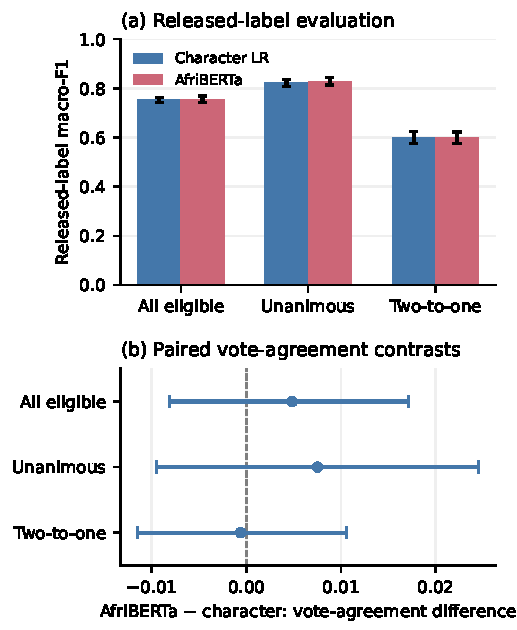
\includegraphics[width=\columnwidth]{images/agreement_evaluation.pdf}
\caption{Released-label macro-F1 and paired vote-agreement contrasts.
All-eligible results include the displayed subgroups, so bars are not
independent samples. Error bars are exploratory, unadjusted 95\% intervals.
The three-way group is omitted because $n=6$.}
\label{fig:agreement}
\end{figure}

\subsection{Released Labels and Raw Majorities}
Of 4,556 eligible posts with a unique raw-vote majority, 4,492 released labels
agree with that majority and 64 differ (1.4\%). The differences occur on
59 two-to-one and five unanimous posts. The remaining six posts have no
unique majority. These are release-consistency observations, not identified
annotation errors. The present files do not establish whether adjudication,
release processing, or another mechanism explains each difference.
NaijaSenti's documented adjudication process makes raw-majority differences
plausible~\cite{naijasenti}, but it does not explain each case in this release.

\subsection{Coverage and Reference Sensitivity}
The full 5,303-post test set ranks word LR (0.7320 macro-F1) above
mBERT (0.7289), whereas the eligible subset reverses their order
(0.7263 versus 0.7296). On the 741 excluded posts, their macro-F1 scores are
0.7473 and 0.6902. Character LR scores 0.7388 on that complement.
These point comparisons show that eligibility can change model ordering;
our unchanged metric ranking applies within the fixed eligible population.
Macro-F1 is recomputed on each subset, not averaged across subset scores.

Restricting the eligible population to the 4,492 posts where the released
label equals the unique raw majority preserves the eligible overall model
ordering under both metrics. AfriBERTa reaches macro-F1 0.7605 and
$V=0.7270$, compared with 0.7570 and 0.7225 for character LR.
The small point advantage therefore persists when the 64 differing labels
and six ties are excluded, but these descriptive checks do not establish
statistical significance or justify correcting any released label.

\section{Discussion}
Retaining individual votes changes what the evaluation can describe, but
does not necessarily change the best-ranked model. Here, both metrics preserve
the overall ordering within the eligible population, while contested posts produce small, uncertain changes
near the top. The evidence supports a more explicit description of evaluation
conditions, not a claim that an alternative metric reveals a decisive winner.

Lower macro-F1 on contested posts is an association with observed disagreement.
It does not show that disagreement causes model errors or that these posts
are intrinsically ambiguous. Class composition, topic and text length may
differ between groups. Nor can the vote-agreement gap across groups alone
demonstrate poorer understanding: its attainable ceiling differs by design.
The fixed three-epoch encoder budget also does not establish each
architecture's best achievable performance.

The 64 majority/released-label differences demonstrate why votes and final
labels should be distinguished in reproducibility records. Replacing released
labels with raw majorities without a documented rationale could discard
adjudication decisions. We preserve both sources rather than choosing the
reference that gives a preferred model a higher score.

\subsection{Scope and Limitations}
The analysis is a selected, 4,562-post subset of one released Hausa benchmark.
Excluding mixed, indeterminate, missing-vote and unmatched cases may remove
particularly difficult or different examples. Three votes do not characterize
the population of possible interpretations. Post-bootstrap intervals do not
model repeated annotators' dependence across posts, uncertainty in their
population, or model training beyond the three observed seeds.

Only hard predictions were saved for this analysis. We cannot assess
probability calibration, distributional cross-entropy, or whether model
confidence detects disagreement. The six three-way examples are too few
for subgroup inference. This secondary analysis follows inspection of the
whole-test benchmark and is exploratory. It does not verify token-level
code-switching or pragmatic categories and makes no such claims.

\subsection{Ethics and Reproducibility}
The official GitHub release README states CC BY 4.0, while the related
HausaNLP NaijaSenti Hugging Face card states CC BY-NC-SA 4.0.
Release-specific provenance is retained, and public redistribution is
deferred pending clarification. The local Kaggle input metadata records a
private research copy; current remote access permissions have not been
independently rechecked for this audit.
Raw texts and annotation joins are excluded from version control. No new
reviewers are recruited, interviewed or asked to annotate. The reused source
votes are not described as newly collected judgments, and annotator IDs are
used only for within-post distinctness checks, not demographic inference.

The source manifest, exclusion ledger, split hashes, per-item predictions,
model-selection grid, and analysis code form the reproducibility record.
The sharing package contains code, aggregate scores, paper assets, source
checksums, and run metadata. It omits raw posts, annotator records and
per-item outputs. Figures and tables can be regenerated from the packaged
aggregates; exact score recomputation additionally requires the separately
obtained source files and saved predictions identified by their checksums.
The join ledger, vote eligibility rules and released-label/vote distinctions
are additional parts of the reproducibility record. The protocol was recorded
before computing the subgroup model results, after earlier benchmark inspection;
it is not a preregistered confirmatory study.

\section{Conclusion}
We re-evaluate fixed Hausa sentiment predictions against both released labels
and the existing individual votes. Overall point ordering is unchanged between
the two metrics within the eligible subset; coverage filtering changes the
word-LR/mBERT point ordering relative to the full test set.
Contested posts yield small subgroup ordering changes without a reliable
AfriBERTa--character advantage. The audit also identifies 64 released labels
that differ from unique raw majorities. Reporting annotation coverage, vote
patterns, metric ceilings and paired uncertainty provides a reproducible
account of these findings without collecting new participant data.


\begin{thebibliography}{10}
\bibitem{naijasenti}
S.~H.~Muhammad et al.
\newblock NaijaSenti: A Nigerian Twitter Sentiment Corpus for Multilingual
Sentiment Analysis.
\newblock In \emph{Proceedings of LREC}, pp.~590--602, 2022.
\newblock \url{https://aclanthology.org/2022.lrec-1.63/}.

\bibitem{afrisenti}
S.~H.~Muhammad et al.
\newblock AfriSenti: A Twitter Sentiment Analysis Benchmark for African Languages.
\newblock In \emph{Proceedings of EMNLP}, pp.~13968--13981, 2023.
\newblock \url{https://aclanthology.org/2023.emnlp-main.862/}.

\bibitem{hausa2025}
Y.~Aliyu et al., ``Deep learning techniques for sentiment analysis in code-switched
Hausa-English tweets.''
\newblock \emph{International Journal of Information Management Data Insights},
5(1), 100330, 2025.
\newblock \url{https://doi.org/10.1016/j.jjimei.2025.100330}.

\bibitem{le-wi-di}
A.~Uma et al., ``SemEval-2021 Task 12: Learning with Disagreements,''
in \emph{Proceedings of SemEval}, pp.~338--347, 2021.
\url{https://aclanthology.org/2021.semeval-1.41/}.

\bibitem{softlearning}
T.~Fornaciari et al., ``Beyond Black \& White: Leveraging Annotator Disagreement
via Soft-Label Multi-Task Learning,'' in \emph{NAACL}, pp.~2591--2597, 2021.
\url{https://aclanthology.org/2021.naacl-main.204/}.

\bibitem{softmetrics}
G.~Rizzi et al., ``Soft metrics for evaluation with disagreements: an assessment,''
in \emph{NLPerspectives}, pp.~84--94, 2024.
\url{https://aclanthology.org/2024.nlperspectives-1.9/}.

\bibitem{le-wi-di-2023}
E.~Leonardelli et al., ``SemEval-2023 Task 11: Learning with Disagreements
(LeWiDi),'' in \emph{Proceedings of SemEval}, 2023.
\url{https://aclanthology.org/2023.semeval-1.314/}.

\bibitem{le-wi-di-2025}
E.~Leonardelli et al., ``LeWiDi-2025 at NLPerspectives: Third Edition of the
Learning with Disagreements Shared Task,'' in \emph{Proceedings of the 4th
Workshop on Perspectivist Approaches to NLP}, 2025.
\url{https://aclanthology.org/2025.nlperspectives-1.16/}.

\bibitem{clustering2026}
T.~D.~Belay et al., ``Beyond Majority Voting: Agreement-Based Clustering to
Model Annotator Perspectives in Subjective NLP Tasks,''
\emph{arXiv preprint arXiv:2605.09955}, 2026.
\url{https://arxiv.org/abs/2605.09955}.

\bibitem{afriberta-model}
K.~Ogueji, Y.~Zhu, and J.~Lin, ``Small Data? No Problem! Exploring the
Viability of Pretrained Multilingual Language Models for Low-resourced
Languages,'' in \emph{Proceedings of MRL}, 2021.
\url{https://aclanthology.org/2021.mrl-1.11/}.

\bibitem{xlmr-model}
A.~Conneau et al., ``Unsupervised Cross-lingual Representation Learning at
Scale,'' in \emph{Proceedings of ACL}, 2020.
\url{https://aclanthology.org/2020.acl-main.747/}.

\bibitem{bert-model}
J.~Devlin et al., ``BERT: Pre-training of Deep Bidirectional Transformers for
Language Understanding,'' in \emph{Proceedings of NAACL-HLT}, 2019.
\url{https://aclanthology.org/N19-1423/}.
\end{thebibliography}
\end{document}
